\documentclass[aspectratio=169,11pt]{beamer}

% Shared style (ib-tutorials.sty at the repo root).
\makeatletter\def\input@path{{./}{../}}\makeatother
\usepackage{ib-tutorials}

\usepackage[utf8]{inputenc}
\usepackage{amsmath,amssymb}
\usepackage{booktabs}
\usepackage{array}
\newcolumntype{L}[1]{>{\raggedright\arraybackslash}p{#1}}
\usepackage{graphicx}
\graphicspath{{../pictures/3-ibamr-fundamentals/}{pictures/3-ibamr-fundamentals/}}
\usepackage{xcolor}
\usepackage{listings}
\usepackage{tikz}
\usetikzlibrary{arrows.meta,positioning,shapes.geometric,fit,calc,decorations.pathmorphing}
\usepackage{hyperref}

\newcommand{\sourcecredit}[1]{\vfill\begin{flushright}\tiny\textcolor{DarkGray}{#1}\end{flushright}}

\lstset{
  basicstyle=\ttfamily\scriptsize\color{BlackGray},
  keywordstyle=\color{NavyBlue}\bfseries,
  commentstyle=\color{DarkGray}\itshape,
  stringstyle=\color{OliveGreen},
  showstringspaces=false,
  columns=fullflexible,
  keepspaces=true,
  breaklines=true,
  breakindent=1em,
  frame=single,
  framerule=0.4pt,
  rulecolor=\color{LightGray},
  backgroundcolor=\color{LightGray!30},
  xleftmargin=0.25em,
  xrightmargin=0.25em
}
\lstdefinestyle{shell}{morecomment=[l]{\#}}
\lstdefinestyle{input}{morecomment=[l]{//}}
\lstdefinestyle{matlab}{morecomment=[l]{\%}}
\lstdefinestyle{python}{morecomment=[l]{\#}}
\lstdefinestyle{data}{}
\lstdefinestyle{tiny}{basicstyle=\ttfamily\tiny\color{BlackGray}}
\lstdefinestyle{inputtiny}{morecomment=[l]{//},basicstyle=\ttfamily\tiny\color{BlackGray}}
\lstdefinestyle{cpp}{language=C++,morecomment=[l]{//}}
\lstdefinestyle{cpptiny}{language=C++,morecomment=[l]{//},basicstyle=\ttfamily\tiny\color{BlackGray}}
\lstdefinestyle{cmake}{morecomment=[l]{\#}}
\lstdefinestyle{cppmicro}{language=C++,morecomment=[l]{//},basicstyle=\ttfamily\fontsize{5.2}{6.2}\selectfont\color{BlackGray}}

\title[Target points and springs]{Target points, springs and multiple boundaries}
\subtitle{Prescribing motion by moving target points, changing springs in time, and running several structures at once}
\author[Miller]{Laura A. Miller}
\institute[UArizona]{Department of Mathematics, University of Arizona}
\date{Using IB Software \textbullet\ Part III \textbullet\ Chapter 9a}

\begin{document}

% 1
\begin{frame}[plain]
\maketutorialtitlepanel{%
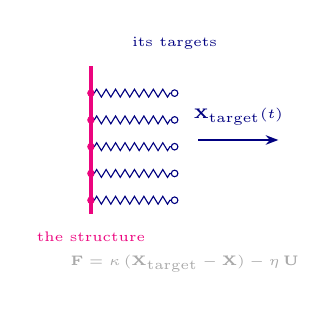
\begin{tikzpicture}[scale=0.85]
  \draw[RubineRed,very thick] (0.4,0) -- (0.4,2.2);
  \foreach \y in {0.2,0.6,...,2.0}{\fill[RubineRed] (0.4,\y) circle (1.6pt);}
  \foreach \y in {0.2,0.6,...,2.0}{\draw[decorate,decoration={zigzag,segment length=1.2mm,amplitude=0.5mm},NavyBlue] (0.45,\y) -- (1.6,\y); \draw[NavyBlue,fill=white] (1.65,\y) circle (1.4pt);}
  \draw[-{Stealth[length=1.6mm]},NavyBlue,thick] (2.0,1.1) -- (3.2,1.1);
  \node[font=\tiny,text=NavyBlue] at (2.6,1.45) {$\mathbf{X}_{\mathrm{target}}(t)$};
  \node[font=\tiny,text=RubineRed] at (0.4,-0.35) {the structure};
  \node[font=\tiny,text=NavyBlue] at (1.65,2.55) {its targets};
  \node[font=\tiny,text=DarkGray] at (1.8,-0.75) {$\mathbf{F} = \kappa\,(\mathbf{X}_{\mathrm{target}} - \mathbf{X}) - \eta\,\mathbf{U}$};
\end{tikzpicture}}
\end{frame}

% 2
\begin{frame}{Learning goals}
\label{fr:goals}
\small By the end of this chapter you should be able to:
\begin{enumerate}
  \item say what a target point and a spring do inside IBAMR (the force laws, where their parameters live at run time, which point ``owns'' a spring);
  \item write a function that moves target points along a prescribed path, call it from \code{main.cpp} before each time step, and build the program with the extra source file;
  \item write the same kind of function for springs: change rest lengths or stiffnesses in time, correctly (through a reference, not a copy);
  \item run several structures in one simulation, find each one's range of point indices, and move them differently;
  \item read the three examples that do this (IB/04 moving cylinders, IB/06 growing springs, IB/07 moving plates), check that a prescribed motion is being followed, and recognize the mistakes that make it silently fail.
\end{enumerate}
\begin{punchbox}
\footnotesize Chapter 9b continues with forces you write yourself (custom spring laws, applied external forces, active pumping). Chapter 10 is beams and curvature. Chapter 6 has the file formats; chapter 8a the stiffness estimates; chapter 11 the forces that come out.
\end{punchbox}
\end{frame}

% 3
\begin{frame}{How this chapter was checked}
\label{fr:checked}
\begin{itemize}\footnotesize
  \item Every class and function named here was checked against the IBAMR 0.19.0 headers (\code{IBTargetPointForceSpec.h}, \code{IBSpringForceSpec.h}, \code{LDataManager.h}, \code{LMesh.h}, \code{LNode.h}); the 2012--2020 lectures' older spellings are listed on slide \ref{fr:api} so that old code can be read.
  \item The three examples (IB/04, IB/06, IB/07) build with 0 warnings on IBAMR 0.16.0 and 0.19.0 and ran to the end; the figures are from their shipped runs, analysed from the \code{hier\_data} position files with \code{tools/ch9a\_figures.py}.
  \item The one real bug in the course material (a rest length changed on a copy, so the springs never grew) is explained on slide \ref{fr:copybug} and fixed in IB/06; the READMEs record the measured time-step limits and the motions.
  \item The 2015--2020 statements about multiple boundaries (``I don't think you can connect springs between them'') are checked against the 0.19.0 initializer on slide \ref{fr:connect}.
\end{itemize}
\begin{punchbox}
\footnotesize Slide numbers refer to this deck; chapter numbers (3, 5, 6, 7, 8a, 8b, 9b, 10, 11, 13, 16) to the other chapters of this series.
\end{punchbox}
\end{frame}

% 4
\begin{frame}{Where to look things up}
\label{fr:lookup}
\small
\begin{itemize}
  \item \al{The header of \code{LDataManager}} (\code{ibtk/include/ibtk/LDataManager.h}) carries, in its documentation comment, a complete worked example of moving target points and one of reading the points' positions: the modern reference for everything in this chapter (slides \ref{fr:loop}, \ref{fr:positions}).
  \item \al{The force-spec headers}: \code{include/ibamr/IBTargetPointForceSpec.h}, \code{IBSpringForceSpec.h}, \code{IBBeamForceSpec.h}: what each object stores and the accessors that return references (slide \ref{fr:specs}).
  \item \al{The examples of this series}: IB/04 (one structure, moving targets), IB/07 (two structures, moving targets), IB/06 (springs changed in time); each has its \code{update\_*.cpp}, \code{.h}, the \code{main.cpp} hook and a README with the measured facts.
  \item \al{The IBAMR FAQ} on the wiki, \url{https://github.com/IBAMR/IBAMR/wiki/FAQ}: the 2012 answers quoted on slide \ref{fr:faq} came from its predecessor.
  \item The 2013 slides pointed to the Google Code source browser and class pages, and to course servers (sakai, nemo); all gone. The class documentation is now generated from the headers (\url{https://ibamr.github.io/docs}).
\end{itemize}
\end{frame}

% 5
\begin{frame}[fragile]{Target points and springs, as IBAMR sees them at run time}
\label{fr:specs}
\begin{columns}[T,onlytextwidth]
\begin{column}{0.52\textwidth}
\footnotesize The files of chapter 6 are read once, at start-up, by \code{IBStandardInitializer}. From then on each element lives in a small object attached to one Lagrangian point, its \al{master} point:
\begin{itemize}
  \item \code{IBTargetPointForceSpec}: for a target point, its stiffness $\kappa$, damping $\eta$ and \al{target position} $\mathbf{X}_{\mathrm{target}}$ (initially the point's own position). Force $\kappa\,(\mathbf{X}_{\mathrm{target}} - \mathbf{X}) - \eta\,\mathbf{U}$: ``a penalty force that approximately imposes a Dirichlet boundary condition at a single node'' (the header).
  \item \code{IBSpringForceSpec}: for the lower-numbered end of each spring, the list of its springs: the other end's index, the force-function index, and a parameter vector per spring, by convention \code{[0]} the stiffness and \code{[1]} the rest length. ``Springs now have an arbitrary number of parameters'' (2020).
  \item \code{IBBeamForceSpec}: the neighbour pairs, bending rigidities and preferred curvatures (chapter 10).
\end{itemize}
\end{column}
\begin{column}{0.46\textwidth}
\begin{lstlisting}[style=cpptiny]
// IBTargetPointForceSpec (0.19.0): the accessors return references
int&         getMasterNodeIndex();
double&      getStiffness();
double&      getDamping();
IBTK::Point& getTargetPointPosition();

// IBSpringForceSpec
unsigned int                      getNumberOfSprings() const;
int&                              getMasterNodeIndex();
std::vector<int>&                 getSlaveNodeIndices();
std::vector<int>&                 getForceFunctionIndices();
std::vector<std::vector<double>>& getParameters();   // [k][0] stiffness, [k][1] rest length
\end{lstlisting}
\footnotesize Because they return \al{references}, you can change a target position or a rest length in place and the force routine (\code{IBStandardForceGen}, chapter 8b) uses the new value at the next force evaluation. That is the whole mechanism of this chapter. ``You may change the parameter values but must not resize the vectors'' (the header of \code{getParameters}).
\end{column}
\end{columns}
\end{frame}

% 6
\begin{frame}{Three ways to prescribe motion}
\label{fr:ways}
\scriptsize
\begin{tabular}{@{}L{0.2\textwidth}L{0.36\textwidth}L{0.34\textwidth}@{}}
\toprule
Way & How & Use it for\\
\midrule
\al{move the target points} (this chapter) & before each step, shift every $\mathbf{X}_{\mathrm{target}}$ along the path; the tethers drag the structure after them & a rigid or nearly rigid body on a known path: a translating plate, a rotating wing, a pumping wall, a flapping fin (with soft tethers it also bends)\\
\al{change the springs} (this chapter) & before each step, change rest lengths (growth, muscle shortening) or stiffnesses (activation) & structures that change shape from inside: growing fibres, contracting tubes, stiffening or softening tissue\\
\al{apply a force} (chapter 9b) & write a force law or an external body force and register it & muscles with a force--length law, pumping by travelling waves of force, anything that is not a spring\\
\bottomrule
\end{tabular}

\vspace{2mm}
\small All three happen \emph{on the Lagrangian side}: the fluid still sees only a force density spread by the kernel (chapter 5). A moving target point does not set a velocity; it sets a force that pulls the point toward where it should be, so the structure lags its path by $F/\kappa$ and the tether force is the force the fluid exerts on the structure (slide \ref{fr:cyl2}).
\vspace{1mm}

\small The 2014--2020 ``What can go wrong'' advice applies to all three: ramp the motion from rest (chapter 7), and do not make the stiffness larger than the time step can take (slide \ref{fr:dt}).
\end{frame}

% 7
\begin{frame}[fragile]{The 2012 FAQ answers, kept word for word}
\label{fr:faq}
\small \emph{How can I have time-dependent target point locations?} ``Take a look at the \code{moving\_plates} example. This example is for the specific case of time-dependent target point locations. The linked code has a routine (\code{update\_target\_point\_positions}) that loops over the local IB points (i.e., the IB points that are `local to the processor'). The pseudo-code is roughly:''
\begin{lstlisting}[style=data]
for each local IB point {
    check to see if the point has a target point spec
    if yes: update the material properties w/ that target spec
}
\end{lstlisting}
\small ``The properties for the target points are stored in \code{IBTargetPointForceSpec} objects. Functionality has been added to the most recent IBAMR versions to simplify the code required to access these objects. In particular, for each Lagrangian (IB) point, you can do \code{tbox::Pointer<T> spec = node\_idx.getStashData<T>();} to get a pointer to any object of type T that is associated with the Lagrangian point.''
\vspace{1mm}

\footnotesize Today's spelling is \code{node->getNodeDataItem<T>()}, returning a plain pointer (slide \ref{fr:api}); everything else in this answer is still exactly right. The springs' answer is on the next slide.
\end{frame}

% 7b
\begin{frame}{The 2012 FAQ answers, continued: springs}
\label{fr:faq2}
\small \emph{How can I have time-dependent spring constants or resting lengths?} ``If you use class \code{IBStandardInitializer} to initialize the Lagrangian structure and provide a \code{.spring} file, then the first point in each spring will have associated with it an object of type \code{IBSpringForceSpec}. Each spring is associated with ONLY ONE of the two ends of the spring. By default, this is the `master' point index, which is simply the lower of the two indices. This means that it is possible for some IB points not to have any force spec objects, even though those points might be connected to another point by a spring (or a beam). If there are not any objects of a specified type T associated with a particular node, then \code{getStashData<T>()} will return a null pointer. You should always check to see if the returned pointer is non-null before trying to do anything with it.''
\vspace{1mm}

\small ``To update the properties of the objects that describe the springs will require a function similar to the \code{update\_target\_point\_positions} function. Refer to the documentation for class \code{IBSpringForceSpec} to see what properties you can access and modify.''
\vspace{1mm}

\footnotesize Still exactly right, with \code{getNodeDataItem} for \code{getStashData} and \code{getParameters()} for the properties (slides \ref{fr:specs}, \ref{fr:springs}). The one thing the answer does not say, because it was not yet a problem, is that the property must be changed \emph{in place} (slide \ref{fr:copybug}).
\end{frame}

% 8
\begin{frame}[fragile]{Where the update is called: the time loop in \code{main.cpp}}
\label{fr:hook}
\begin{columns}[T,onlytextwidth]
\begin{column}{0.54\textwidth}
\begin{lstlisting}[style=cpptiny]
// IB/04 main.cpp, inside the time loop (condensed)
while (!MathUtilities<double>::equalEps(loop_time, loop_time_end) &&
       time_integrator->stepsRemaining())
{
    iteration_num = time_integrator->getIntegratorStep();
    loop_time     = time_integrator->getIntegratorTime();
    dt = time_integrator->getMaximumTimeStepSize();

    // Move the cylinders' target points to where they should be at the
    // end of this time step (update_target_point_positions.cpp).
    LDataManager* l_data_manager = ib_method_ops->getLDataManager();
    update_target_point_positions(patch_hierarchy, l_data_manager, loop_time, dt);

    time_integrator->advanceHierarchy(dt);
    loop_time += dt;
    ...
}
\end{lstlisting}
\begin{lstlisting}[style=cmake]
# CMakeLists.txt: both source files, or the link step fails
add_executable(main2d main.cpp update_target_point_positions.cpp)
\end{lstlisting}
\end{column}
\begin{column}{0.44\textwidth}
\scriptsize The program is IB/01's (chapter 3) plus one call per step, placed \al{before} \code{advanceHierarchy}: the targets are moved to where they should be at the end of the step, and the step then pulls the structure after them.
\begin{itemize}
  \item \code{ib\_method\_ops->getLDataManager()} hands over the object that owns the Lagrangian data on every level.
  \item \code{loop\_time} is the time at the start of the step and \code{dt} the step the integrator is about to take; the function receives both.
  \item ``You also need to add these files to \code{main.C}'' (2015--2020): today that is the \code{\#include} of the header in \code{main.cpp} and the extra file in \code{add\_executable}. Leave it out and the link fails with \code{undefined reference to} \code{`update\_target\_point\_positions'}.
\end{itemize}
\scriptsize An alternative that needs no edit of the loop: register the function as a callback with \code{time\_integrator->}\allowbreak\code{registerPreprocess}\allowbreak\code{IntegrateHierarchyCallback(...)} (\code{HierarchyIntegrator.h}); the examples keep the explicit call because it is easier to read.
\end{column}
\end{columns}
\end{frame}

% 9
\begin{frame}[fragile]{The function's signature and what you get}
\label{fr:signature}
\begin{columns}[T,onlytextwidth]
\begin{column}{0.5\textwidth}
\begin{lstlisting}[style=cpptiny]
// update_target_point_positions.h (IB/04; the whole header)
#ifndef included_update_target_point_positions
#define included_update_target_point_positions
// IBAMR 0.16 needs LData.h for LDataManager.h to compile; 0.19 does not.
#include <ibtk/LData.h>
#include <ibtk/LDataManager.h>
#include <PatchHierarchy.h>

void update_target_point_positions(
    SAMRAI::tbox::Pointer<SAMRAI::hier::PatchHierarchy<NDIM> > hierarchy,
    IBTK::LDataManager* l_data_manager,
    double current_time,
    double dt);
#endif
\end{lstlisting}
\footnotesize ``You have access to the \code{current\_time} and time step (\code{dt}). You also have access to the patch hierarchy and can get the nodes the particular processor is working on.'' (2015--2020)
\end{column}
\begin{column}{0.48\textwidth}
\scriptsize The four arguments:
\begin{itemize}
  \item \code{hierarchy}: the grid; needed only for \code{getFinestLevelNumber()}, because the structure lives on the finest level (the \code{level\_number} of chapter 6);
  \item \code{l\_data\_manager}: gives the Lagrangian mesh of a level (\code{getLMesh}), the index range of each structure (\code{getLagrangianStructureIndexRange}) and the position data (\code{getLData("X", ln)});
  \item \code{current\_time}, \code{dt}: the path is a function of time, and the increment to add this step is (speed at this time) $\times$ \code{dt}.
\end{itemize}
\scriptsize The course header included about twenty IBAMR, SAMRAI and PETSc headers, among them \code{IBAMR\_config.h} and \code{IBTK\_config.h}, which CMake installs do not have, and \code{app\_namespaces.h}, which IBAMR says must never be included from a header. The three above are all it needs (chapter 3's porting checklist).
\end{column}
\end{columns}
\end{frame}

% 10
\begin{frame}[fragile]{The loop over the points}
\label{fr:loop}
\begin{columns}[T,onlytextwidth]
\begin{column}{0.54\textwidth}
\begin{lstlisting}[style=cpptiny]
const int finest_ln = hierarchy->getFinestLevelNumber();

// Structure 0's index range [first, second)
const std::pair<int, int> cyl_lag_idxs =
    l_data_manager->getLagrangianStructureIndexRange(0, finest_ln);

// The Lagrangian mesh of the finest level: local nodes AND ghost nodes
Pointer<LMesh> mesh = l_data_manager->getLMesh(finest_ln);
std::vector<LNode*> nodes = mesh->getLocalNodes();
nodes.insert(nodes.end(), mesh->getGhostNodes().begin(), mesh->getGhostNodes().end());

for (LNode* const node : nodes)
{
    IBTargetPointForceSpec* const force_spec = node->getNodeDataItem<IBTargetPointForceSpec>();
    if (force_spec == nullptr) continue;      // not a target point

    const int lag_idx = node->getLagrangianIndex();
    Point& X_target = force_spec->getTargetPointPosition();
    if (cyl_lag_idxs.first <= lag_idx && lag_idx < cyl_lag_idxs.second)
    {
        X_target[1] += (something) * dt;      // the motion goes here
    }
}
\end{lstlisting}
\end{column}
\begin{column}{0.44\textwidth}
\scriptsize Line by line (the 2020 lecture's comments, updated):
\begin{itemize}
  \item \code{getLagrangianStructureIndexRange(0, ln)}: ``the first point on the structure; if you have more than one boundary, you can use this to determine which boundary you are on.'' Half-open: \code{second} is one past the last index.
  \item \code{getLMesh}, \code{getLocalNodes}, \code{getGhostNodes}: the points this process owns \al{and} the copies it holds of neighbours' points. ``In parallel, we also need to update the target point locations of the ghost data'' (the header's example).
\end{itemize}
\scriptsize The rest of the loop is on the next slide.
\end{column}
\end{columns}
\end{frame}

% 10b
\begin{frame}[fragile]{The loop over the points, continued}
\label{fr:loop2}
\begin{columns}[T,onlytextwidth]
\begin{column}{0.5\textwidth}
\begin{lstlisting}[style=cpptiny]
for (LNode* const node : nodes)
{
    IBTargetPointForceSpec* const force_spec = node->getNodeDataItem<IBTargetPointForceSpec>();
    if (force_spec == nullptr) continue;      // not a target point

    const int lag_idx = node->getLagrangianIndex();
    Point& X_target = force_spec->getTargetPointPosition();
    if (cyl_lag_idxs.first <= lag_idx && lag_idx < cyl_lag_idxs.second)
    {
        X_target[1] += (something) * dt;      // the motion goes here
    }
}
\end{lstlisting}
\footnotesize Why the ghosts matter: leave them out and a point near a patch boundary keeps its old target on one process while its copy on the neighbouring process moves. On one process nothing is wrong; in parallel the structure tears or lags at process boundaries, and the symptom appears only on the cluster.
\end{column}
\begin{column}{0.48\textwidth}
\footnotesize
\begin{itemize}
  \item \code{getNodeDataItem<T>()}: ``get data from the target point, such as its position''; \code{nullptr} if the point has no target spec, which is why the test comes first.
  \item \code{getLagrangianIndex()}: the point's number in the files (chapter 6), fixed for the run; the PETSc index, which changes at every regrid, is a different thing (slide \ref{fr:positions}).
  \item \code{Point\& X\_target}: a reference into the spec; \code{X\_target[0]}, \code{[1]}, \code{[2]} are its components, and adding to them changes the stored target.
  \item the range test lets one function serve several structures (slide \ref{fr:multi2}); with one structure it is always true, and the 2020 lecture kept it ``because we only have one wing in this case''.
  \item \code{(something) * dt}: a speed times the step, so that the targets move by the right distance whatever \code{DT} is.
\end{itemize}
\end{column}
\end{columns}
\end{frame}

% 10c
\begin{frame}[fragile]{Reading the points' current positions in code}
\label{fr:positions}
\begin{columns}[T,onlytextwidth]
\begin{column}{0.54\textwidth}
\begin{lstlisting}[style=cpptiny]
// from the LDataManager.h documentation (0.19.0), condensed
void print_eul_data(Pointer<PatchHierarchy<NDIM>> hierarchy, LDataManager* const l_data_manager)
{
    const int finest_ln = hierarchy->getFinestLevelNumber();
    Pointer<LData> X_data = l_data_manager->getLData("X", finest_ln);
    Vec X_vec = X_data->getVec();
    double* x_vals;
    int ierr = VecGetArray(X_vec, &x_vals);
    IBTK_CHKERRQ(ierr);

    Pointer<LMesh> mesh = l_data_manager->getLMesh(finest_ln);
    for (const auto& node : mesh->getLocalNodes())
    {
        const int lag_idx   = node->getLagrangianIndex();
        const int petsc_idx = node->getLocalPETScIndex();   // local, not global
        Eigen::Map<VectorNd> X(&x_vals[petsc_idx * NDIM]);
        pout << "Eulerian location of node " << lag_idx << ":\n" << X << "\n";
    }
    // (restore the array with VecRestoreArray when done)
}
\end{lstlisting}
\end{column}
\begin{column}{0.44\textwidth}
\scriptsize A target point knows where it \emph{should} be; the point's actual position lives in the \code{LData} vector \code{"X"}, a PETSc vector in \al{PETSc ordering}. From the header: ``The Lagrangian ordering is fixed at the beginning of the simulation and is set by the reading of the vertices. The PETSc ordering, however, will change over the course of the simulation. Whenever a regridding operation is triggered, the PETSc indexing is changed to ensure efficient memory usage.''
\begin{itemize}
  \item so a position is reached through the node's \code{getLocalPETScIndex()}, never through its Lagrangian index;
  \item \code{"X"} is the position, \code{"U"} the velocity, \code{"F"} the force, on the same ordering;
  \item uses: a tether law that depends on where the point \emph{is} (chapter 9b), a feedback controller, or a printed check of the lag (slide \ref{fr:check}).
\end{itemize}
\scriptsize For analysis after the run, the \code{X.*} files of chapter 11 are simpler: they are already in Lagrangian order.
\end{column}
\end{columns}
\end{frame}

% 11
\begin{frame}[fragile]{The moving cylinders (IB/04): the motion}
\label{fr:cyl}
\begin{columns}[T,onlytextwidth]
\begin{column}{0.52\textwidth}
\begin{lstlisting}[style=cpptiny]
static const double V = 0.2;           // speed after the ramp (m/s)
static const double time_to_acc = 0.1; // time to accelerate from 0 to V (s)
...
    if (cylinder_lag_idxs.first <= lag_idx && lag_idx < cylinder_lag_idxs.second)
    {
        if (current_time <= time_to_acc)
        {
            X_target[1] += current_time / time_to_acc * V * dt; // speeding up
        }
        else
        {
            X_target[1] += V * dt;                              // constant speed
        }
    }
\end{lstlisting}
\footnotesize The 2015--2020 lecture's gloss: ``check to see if we are in the acceleration phase; check to see if the node is on the first wing (it is, because we only have one wing in this case); determine the new position in the $y$-direction, we aren't moving in the $x$-direction here; here we move the wing at a constant speed.''
\end{column}
\begin{column}{0.46\textwidth}
\scriptsize What the code says:
\begin{itemize}
  \item the targets move in $+y$ at a speed that rises linearly from $0$ to $V$ over \code{time\_to\_acc}, then stays at $V$: a \al{ramp}, for the reason of chapter 7 (no impulsive start);
  \item the increment is a \al{displacement}, speed $\times$ \code{dt}, added to the target each step; the targets are never \emph{set} to a position, only shifted, so the function needs no memory of where they started;
  \item the course comments called the row ``the wing'' and said it moves ``to the left or right'' (it moves up); the series' comments say what the code does.
\end{itemize}
\scriptsize The structure: 9 cylinders of radius 2.5 mm (5 cells across), 33 points each, 0.05 m apart on the $x$ axis, every point a target with $\kappa = 4.1\times10^6$; $\mu = 100$, so $\mathrm{Re} = 0.01$ (chapters 8a, 8b). The README calls them bristles; the course called the row a holey plate.
\end{column}
\end{columns}
\end{frame}

% 12
\begin{frame}{The moving cylinders: do they follow?}
\label{fr:cyl2}
\begin{columns}[T,onlytextwidth]
\begin{column}{0.58\textwidth}
\centering
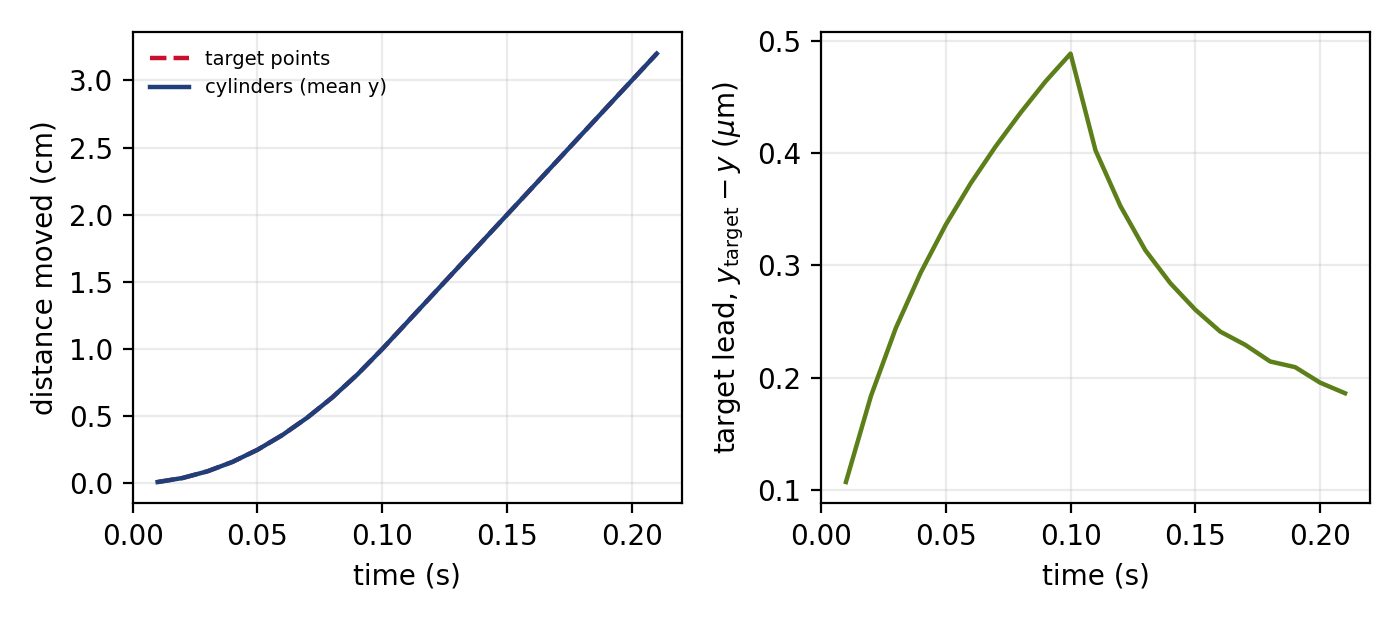
\includegraphics[width=0.96\textwidth]{ch9a-cylinders-lag}
\end{column}
\begin{column}{0.4\textwidth}
\scriptsize From the shipped run (0.2 s, 4 cores): the mean $y$ of the 297 points against the target path. The two curves lie on top of each other; the right panel is their difference.
\begin{itemize}
  \item the lead of the targets peaks at $0.48\ \mu$m at the end of the ramp and settles to $0.2\ \mu$m: a \al{five-thousandth of a cell} ($\Delta x = 1/1024$ m);
  \item the lead is the force the fluid exerts on the row divided by $\kappa$: with $\kappa = 4.1\times10^6$ per point, a drag of a fraction of a newton per metre per point is a fraction of a micrometre. \code{integral\{F\}} prints that force (chapter 11): $249.6$ N/m in $y$ at $t = 0.19$ s, $238.9$ at the end of the run ($0.2$ s);
  \item the peak at $t = 0.1$ s is the acceleration reaction: the fluid resists the change of speed, not the speed.
\end{itemize}
\scriptsize The price of following this closely is the time step: $\kappa = 4.1\times10^6$ needs \code{DT = 2e-5} (slide \ref{fr:dt}).
\end{column}
\end{columns}
\sourcecredit{IB/04 with IBAMR 0.19.0, shipped input; \code{tools/ch9a\_figures.py} reads \code{hier\_data\_IB2d/X.*} and the \code{.vertex} file (the positions at $t = 0$).}
\end{frame}

% 13
\begin{frame}{One API across four versions}
\label{fr:api}
\footnotesize The 2012--2020 slides show the same function in three dialects, and the comments say ``depending on the version of IBAMR, you need to select one of the ways''. The spellings, oldest first:

\tiny
\begin{tabular}{@{}L{0.22\textwidth}L{0.32\textwidth}L{0.36\textwidth}@{}}
\toprule
What & 2009--2013 (Griffith's \code{moving\_plates}, the 2012 deck) & 2015--2020 courses $\rightarrow$ 0.19.0 (this series)\\
\midrule
iterate over the points & \code{LNodeIndexData} on each patch: \code{for (PatchLevel::Iterator p(level); ...) ... idx\_data->lnode\_index\_begin(patch\_box)} & \code{mesh->getLocalNodes()} plus \code{getGhostNodes()} from \code{l\_data\_manager->getLMesh(ln)}\\
the point & \code{const LNodeIndex\& node\_idx = *it} & \code{LNode* node}\\
the spec & \code{tbox::Pointer<T> spec = node\_idx.getStashData<T>()}; test \code{!spec.isNull()} & \code{T* spec = node->getNodeDataItem<T>()}; test \code{spec != nullptr}\\
the target position & \code{std::vector<double>\& X\_target}, then \code{TinyVector<double,NDIM>\&}, then \code{IBTK::Vector<double,NDIM>\&} & \code{IBTK::Point\& X\_target = spec->getTargetPointPosition()} (an Eigen vector)\\
a spring's rest length & \code{spec->getRestingLengths()[k]}, stiffness \code{getStiffnesses()[k]} & \code{spec->getParameters()[k][1]}, stiffness \code{[k][0]}\\
source file & \code{update\_target\_point\_positions.C}, Makefile & \code{.cpp}, CMake (chapter 3)\\
\bottomrule
\end{tabular}

\footnotesize Old code found on a disk or in a thesis is worth reading for its \emph{motion}; port the mechanics with this table and chapter 3's checklist. The 2009 version (next slide, and in full in the archive, Part X) did two things the course versions later fixed: it did not ramp the speed (the plates started at $V = 0.1$ m/s instantly), and it did not visit ghost nodes (its patch iteration covers only the interior of each patch).
\end{frame}

% 14
\begin{frame}[fragile]{The oldest version (2009), for reading old code}
\label{fr:old}
\begin{columns}[T,onlytextwidth]
\begin{column}{0.64\textwidth}
\begin{lstlisting}[style=cppmicro]
// Created on 06 Oct 2009 by Boyce Griffith; shown in the January 2012 tutorial
const int lag_node_index_idx = lag_manager->getLNodeIndexPatchDescriptorIndex();
tbox::Pointer<hier::PatchLevel<NDIM> > level = hierarchy->getPatchLevel(finest_ln);
for (SAMRAI::hier::PatchLevel<NDIM>::Iterator p(level); p; p++)
{
    SAMRAI::tbox::Pointer<SAMRAI::hier::Patch<NDIM> > patch = level->getPatch(p());
    const SAMRAI::hier::Box<NDIM>& patch_box = patch->getBox();
    const SAMRAI::tbox::Pointer<LNodeIndexData> idx_data = patch->getPatchData(lag_node_index_idx);
    for (LNodeIndexData::LNodeIndexIterator it = idx_data->lnode_index_begin(patch_box);
         it != idx_data->lnode_index_end(); ++it)
    {
        const LNodeIndex& node_idx = *it;
        const int lag_idx = node_idx.getLagrangianIndex();
        SAMRAI::tbox::Pointer<IBTargetPointForceSpec> force_spec = node_idx.getStashData<IBTargetPointForceSpec>();
        if (!force_spec.isNull())
        {
            std::vector<double>& X_target = force_spec->getTargetPointPosition();
            if (plate2d_left_lag_idxs.first <= lag_idx && lag_idx < plate2d_left_lag_idxs.second) X_target[0] -= dt*V;
            if (plate2d_rght_lag_idxs.first <= lag_idx && lag_idx < plate2d_rght_lag_idxs.second) X_target[0] += dt*V;
        }
    }
}
\end{lstlisting}
\end{column}
\begin{column}{0.34\textwidth}
\scriptsize The same algorithm as slide \ref{fr:loop}: find the index ranges, visit every point, test for a target spec, shift the target. The differences are all in how the points are reached (patch by patch, through the \code{LNodeIndexData} patch data) and in the smart-pointer types.
\vspace{1mm}

\scriptsize The 2012 deck also quoted the file formats of chapter 6 as they then were: ``the rest length and force function index are optional; by default the rest length is 0.0'' was true then, and is not now (chapter 6: the rest length is required).
\end{column}
\end{columns}
\end{frame}

% 15
\begin{frame}[fragile]{Changing springs in time: the growing fibre (IB/06)}
\label{fr:springs}
\begin{columns}[T,onlytextwidth]
\begin{column}{0.52\textwidth}
\begin{lstlisting}[style=cpptiny]
// update_springs.cpp (IB/06), the loop
static const double growth_rate = 0.01;   // how fast each rest length grows (m/s)

Pointer<LMesh> mesh = l_data_manager->getLMesh(finest_ln);
std::vector<LNode*> nodes = mesh->getLocalNodes();
nodes.insert(nodes.end(), mesh->getGhostNodes().begin(), mesh->getGhostNodes().end());

for (LNode* const node : nodes)
{
    IBSpringForceSpec* const spring_spec = node->getNodeDataItem<IBSpringForceSpec>();
    if (spring_spec == nullptr) continue;   // not the master of any spring

    // spring[0] is the stiffness and spring[1] is the rest length. The &
    // makes "spring" a reference to the numbers stored in the spec.
    for (std::vector<double>& spring : spring_spec->getParameters())
    {
        spring[1] += growth_rate * dt;
    }
}
\end{lstlisting}
\end{column}
\begin{column}{0.46\textwidth}
\scriptsize ``The resting lengths of a 2D fiber are increased at each time step. New files are \code{update\_springs.C} and \code{update\_springs.h}. The idea is similar to \code{update\_target\_point\_positions}.'' (2015--2020; the course's \code{Example\_2DSprings}.)
\begin{itemize}
  \item the loop is the target-point loop with \code{IBSpringForceSpec} in place of the target spec;
  \item a point without a spec is not the \emph{master} of any spring (the last point of the fibre); it is still the far end of one;
  \item \code{getParameters()} is a vector of vectors, one per spring the point masters; the inner loop changes \al{every} spring of the point. The course version changed only \code{[0]}, which is the same thing on a fibre where each point masters one spring, and wrong on a network;
  \item the \al{reference} \code{std::vector<double>\& spring} is the whole point: next slide.
\end{itemize}
\end{column}
\end{columns}
\end{frame}

% 16
\begin{frame}[fragile]{The bug that was in the course code for years}
\label{fr:copybug}
\begin{columns}[T,onlytextwidth]
\begin{column}{0.5\textwidth}
\begin{lstlisting}[style=cpptiny]
// the 2015-2020 slides and the course's update_springs.C
double resting_length = spring_spec->getParameters()[0][1];
// "Get the resting lengths of the springs associated with that node."
resting_length += 0.01*dt;
// "increase the resting length of each spring with speed 0.01."
\end{lstlisting}
\footnotesize \code{double resting\_length = ...} makes a \al{copy} of the number. Adding to the copy changes nothing in the spec, and \code{IBStandardForceGen} keeps reading the old rest length: the springs never grow, the run finishes, and nothing is reported. Every course copy of the example from 2013 to 2020 had this, including the slides; one 2014 edit (``Change 2-14'') fixed it in the code but kept the old lines as comments, so later copies reverted.
\begin{lstlisting}[style=cpptiny]
// the fix: change the stored number through a reference
std::vector<double>& params = spring_spec->getParameters()[0];
params[1] += 0.01*dt;
// or, for every spring of the point, the loop of the previous slide
\end{lstlisting}
\end{column}
\begin{column}{0.48\textwidth}
\scriptsize How to tell, and how to avoid it:
\begin{itemize}
  \item \al{Tell}: the fibre in the course's run did not lengthen; the 2015--2020 ``update\_springs example'' picture (a straight fibre with two symmetric eddies) is what a fibre that does not grow looks like. The series' run (next slide) lengthens six-fold in 0.5 s.
  \item \al{Avoid}: whenever a getter returns a reference (slide \ref{fr:specs}), take it as a reference (\code{T\&} or \code{auto\&}); a plain \code{double} or \code{auto} copies. Check the header: the accessors come in \code{const} and non-\code{const} pairs for exactly this use.
  \item \al{Verify}: a short run and the fibre's length against the sum of rest lengths (the figure of the next slide), or \code{pout} one rest length every few hundred steps.
\end{itemize}
\scriptsize The 2016 ``stretching and shrinking plates'' exercise (slide \ref{fr:stretch}) had the same line, in one version written as \code{resting\_length[0] += ...}, which does not compile with \code{getParameters()}.
\end{column}
\end{columns}
\end{frame}

% 17
\begin{frame}{The growing fibre: what happens}
\label{fr:fibre}
\begin{columns}[T,onlytextwidth]
\begin{column}{0.5\textwidth}
\centering
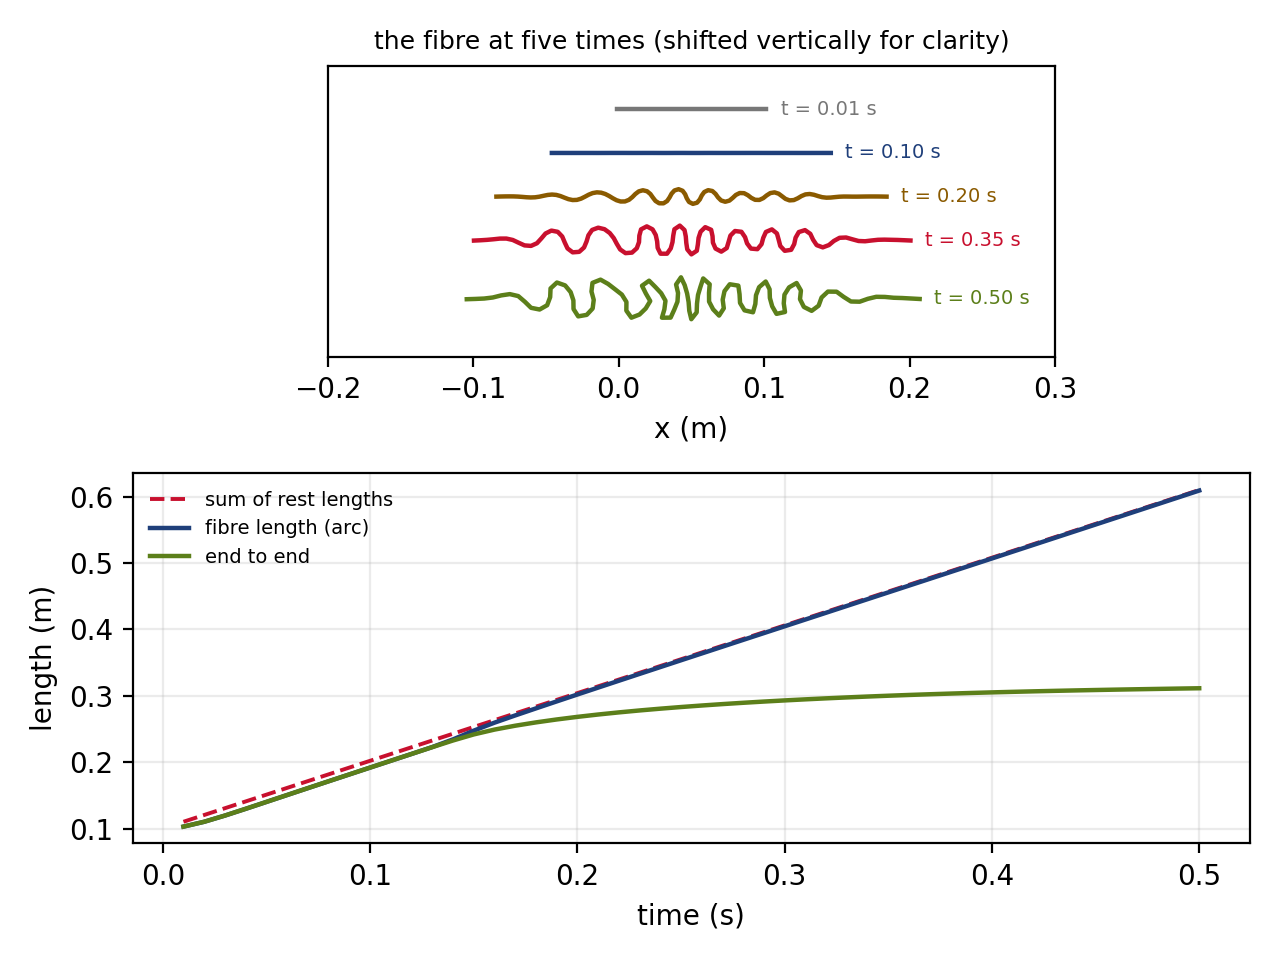
\includegraphics[width=\linewidth,height=0.66\textheight,keepaspectratio]{ch9a-growing-fibre}
\end{column}
\begin{column}{0.48\textwidth}
\scriptsize A straight fibre of 103 points, springs only (no beams, no targets), $K = 2000$, in fluid of viscosity $100$. Every rest length grows at $0.01$ m/s, so the fibre's rest length grows at $1.02$ m/s (102 springs in series, chapter 8b's arithmetic).
\begin{itemize}
  \item for the first $0.15$ s the fibre stays straight and lengthens nearly as fast as its rest lengths grow, pushing fluid out of the way; the springs are compressed by the drag (the arc length lags the rest-length sum by up to 7\%);
  \item then it \al{buckles}: with no bending stiffness, a compressed fibre has no straight equilibrium, and from $0.15$ s on it folds into waves whose wavelength is set by the fluid's resistance, not by the structure;
  \item by $0.5$ s the rest lengths add up to $0.61$ m and the arc length is $0.609$ m (the springs are nearly relaxed), but the fibre spans only $0.31$ m end to end.
\end{itemize}
\scriptsize What to try (README): a slower \code{growth\_rate} (less drag, straight for longer), a stiffer \code{kappa\_spring} (smaller \code{DT}), or beams (chapter 10), which give the buckling a wavelength of their own.
\end{column}
\end{columns}
\sourcecredit{IB/06 with IBAMR 0.19.0, shipped input (0.5 s); \code{tools/ch9a\_figures.py}. The course version ran 2 s with \code{DT = 1e-6}; the series runs 0.5 s at \code{DT = 1e-4}.}
\end{frame}

% 18
\begin{frame}[fragile]{Changing other things in time}
\label{fr:other}
\small The same loop, with other references:
\begin{lstlisting}[style=cpptiny]
// a spring's stiffness (parameter 0), e.g. activation that switches on at t_on
for (std::vector<double>& spring : spring_spec->getParameters())
    spring[0] = (current_time > t_on) ? K_active / ds : K_passive / ds;     // the FILE value, K/ds (chapter 6)

// a target point's stiffness or damping
double& kappa = force_spec->getStiffness();   kappa = ...;
double& eta   = force_spec->getDamping();     eta   = ...;

// release a tether: set its stiffness to zero (the point then moves freely with the fluid)
force_spec->getStiffness() = 0.0;
\end{lstlisting}
\begin{itemize}\footnotesize
  \item IBFE/01, 05, 08 and 12 release their tethers at a given time in the IBFE way (the tether force law tests the time, chapter 15); for IB structures the equivalent is \code{getStiffness() = 0.0} in an update function.
  \item A rest length can be made to oscillate: \code{spring[1] += A * sin(2*PI*f*current\_time) * dt} (the 2018 exercise of chapter 8b, with $A = 0.00049$ per spring for a plate that lengthens 50\% in a second at 1 Hz).
  \item Changing a \al{stiffness} changes the stable time step (chapter 8a); changing a \al{rest length} does not, but a rest length that shrinks past zero turns the spring into a repulsive one with the wrong sign: keep it positive.
  \item Beams: \code{IBBeamForceSpec::getBendingRigidities()} and \code{getMeshDependentCurvatures()} are references too; chapter 10 changes the preferred curvature in time to make a fin flap.
\end{itemize}
\end{frame}

% 19
\begin{frame}{Multiple boundaries: why}
\label{fr:multi}
\small From the 2014--2020 lectures, word for word:
\begin{itemize}
  \item ``The advantage is that you can easily make them do different things.''
  \item ``The disadvantage is that I don't think you can connect springs between them.''
  \item ``However, if you initialize boundaries in the same positions, they will stick together in those positions. This has the effect of gluing different boundaries or parts of boundaries together.''
  \item ``You can make more than one boundary in IBAMR by creating additional \code{.spring}, \code{.vertex}, \code{.target} files. When you do this, you must add them to the input file.''
\end{itemize}
\vspace{1mm}
\begin{punchbox}
\small Why the glue works: two points at the same place interpolate the \emph{same} fluid velocity (chapter 5) and so move together for ever, exactly, without any force between them. It is a kinematic weld, not a joint: it transmits displacement, and the forces each structure applies are simply added onto the same fluid. It fails only if the two points are ever at different places, which the interpolation prevents (up to round-off, which IBAMR does not accumulate because both see the same velocity field).
\end{punchbox}
\vspace{1mm}
\small Slide \ref{fr:connect} says what 0.19.0 does and does not allow between structures. First, the mechanics.
\end{frame}

% 20
\begin{frame}[fragile]{Multiple boundaries: the input block and the global numbering}
\label{fr:multi2}
\begin{columns}[T,onlytextwidth]
\begin{column}{0.5\textwidth}
\begin{lstlisting}[style=input]
IBStandardInitializer {
   max_levels = MAX_LEVELS
   structure_names = "plate2d_left_512" , "plate2d_rght_512"
   plate2d_left_512 {
      level_number = MAX_LEVELS - 1        // the finest grid level
   }
   plate2d_rght_512 {
      level_number = MAX_LEVELS - 1
   }
}
\end{lstlisting}
\begin{lstlisting}[style=cpptiny]
// update_target_point_positions.cpp (IB/07): one range per structure
const std::pair<int, int> plate2d_left_lag_idxs = l_data_manager->getLagrangianStructureIndexRange(0, finest_ln);
const std::pair<int, int> plate2d_rght_lag_idxs = l_data_manager->getLagrangianStructureIndexRange(1, finest_ln);
\end{lstlisting}
\end{column}
\begin{column}{0.48\textwidth}
\footnotesize
\begin{itemize}
  \item each structure has its own set of files (\code{plate2d\_left\_512.vertex}, \code{.spring}, \code{.beam}, \code{.target}, and the same for \code{rght}) and its own sub-block with a \code{level\_number} (chapter 6);
  \item \al{the order of \code{structure\_names} is the order of the structures}: structure 0, structure 1, \ldots, and the order of the global point numbers. Point numbers start at 0 in each structure's files; IBAMR numbers all points together in that order, so the left plate's points are 0--102 and the right plate's are 103--205 (README).
\end{itemize}
\footnotesize The index ranges that tell them apart: next slide.
\end{column}
\end{columns}
\end{frame}

% 20b
\begin{frame}{Multiple boundaries: the index ranges}
\label{fr:multi3}
\footnotesize
\begin{itemize}
  \item \code{getLagrangianStructureIndexRange(k, ln)} returns structure $k$'s range of global indices on level \code{ln}: ``\code{.first} is the first Lagrangian index for the left plate, \code{.second} is'' one past ``the last''. (The 2020 slide said ``the last''; the header says half-open, and the code's \code{< second} test agrees.)
  \item ``You will need these to determine which boundary you are on'': the test \code{first <= lag\_idx \&\& lag\_idx < second} inside the loop routes each point to its own motion (slide \ref{fr:plates}).
  \item Names are also available: \code{getLagrangianStructureNames(ln)} lists them in order, and \code{getLagrangianStructureIndex(name, ln)} returns the number of a named structure, if you would rather not count on the order of \code{structure\_names}.
  \item The ranges are per \emph{level}: a structure on a coarser level (\code{level\_number} less than the finest, chapter 6) is not in the finest level's mesh at all, and the update function must ask for that level's mesh and ranges instead. The examples put every structure on the finest level.
  \item In parallel every process knows every range (they are global numbers); the loop over local and ghost nodes then visits only the points it holds.
\end{itemize}
\vspace{1mm}
\begin{punchbox}
\small The ranges are also how the \code{X.*} and \code{F.*} files of chapter 11 are read: the left plate's 103 points come first, then the right's, in global order.
\end{punchbox}
\end{frame}

% 21
\begin{frame}[fragile]{Moving two plates apart (IB/07)}
\label{fr:plates}
\begin{columns}[T,onlytextwidth]
\begin{column}{0.5\textwidth}
\begin{lstlisting}[style=cpptiny]
if (current_time <= time_to_acc)
{
    if (plate2d_left_lag_idxs.first <= lag_idx && lag_idx < plate2d_left_lag_idxs.second)
        X_target[0] -= current_time / time_to_acc * V * dt;
    if (plate2d_rght_lag_idxs.first <= lag_idx && lag_idx < plate2d_rght_lag_idxs.second)
        X_target[0] += current_time / time_to_acc * V * dt;
}
else
{
    if (plate2d_left_lag_idxs.first <= lag_idx && lag_idx < plate2d_left_lag_idxs.second)
        X_target[0] -= V * dt;
    if (plate2d_rght_lag_idxs.first <= lag_idx && lag_idx < plate2d_rght_lag_idxs.second)
        X_target[0] += V * dt;
}
\end{lstlisting}
\footnotesize ``This code will check to see if you are on the right plate or left plate, and then move the plate to the left or right, respectively.'' (2015--2020)
\end{column}
\begin{column}{0.48\textwidth}
\scriptsize ``This example considers two plates with bending and stretching stiffness that move apart as a result of moving target points'' (\code{Example\_2Dmoving\_plates}, now IB/07).
\begin{itemize}
  \item two vertical plates $0.1$ m long, $103$ points each, with springs ($K = 2000$), beams ($EI = 5\times10^{-3}$) and a target on every point ($\kappa = 2000/\Delta s$); they start $5$ mm apart, $2.6$ cells;
  \item the left plate's targets move left, the right plate's right, with the same ramp as the cylinders ($V = 0.2$ m/s after $0.1$ s);
  \item the course ran 2 s, by which time each plate had moved $0.39$ m and the two met again through the periodic boundary, $0.22$ m apart; the series runs 1 s.
\end{itemize}
\scriptsize Because they start only $2.6$ cells apart, ``the two plates push and pull the same fluid'' at first (README): the kernel's four-cell footprints overlap, and the flow between them is the sum of both. That is the glue of slide \ref{fr:multi} at work, briefly, between structures that are \emph{not} coincident.
\end{column}
\end{columns}
\end{frame}

% 22
\begin{frame}{The two plates: what happens}
\label{fr:plates2}
\begin{columns}[T,onlytextwidth]
\begin{column}{0.5\textwidth}
\centering
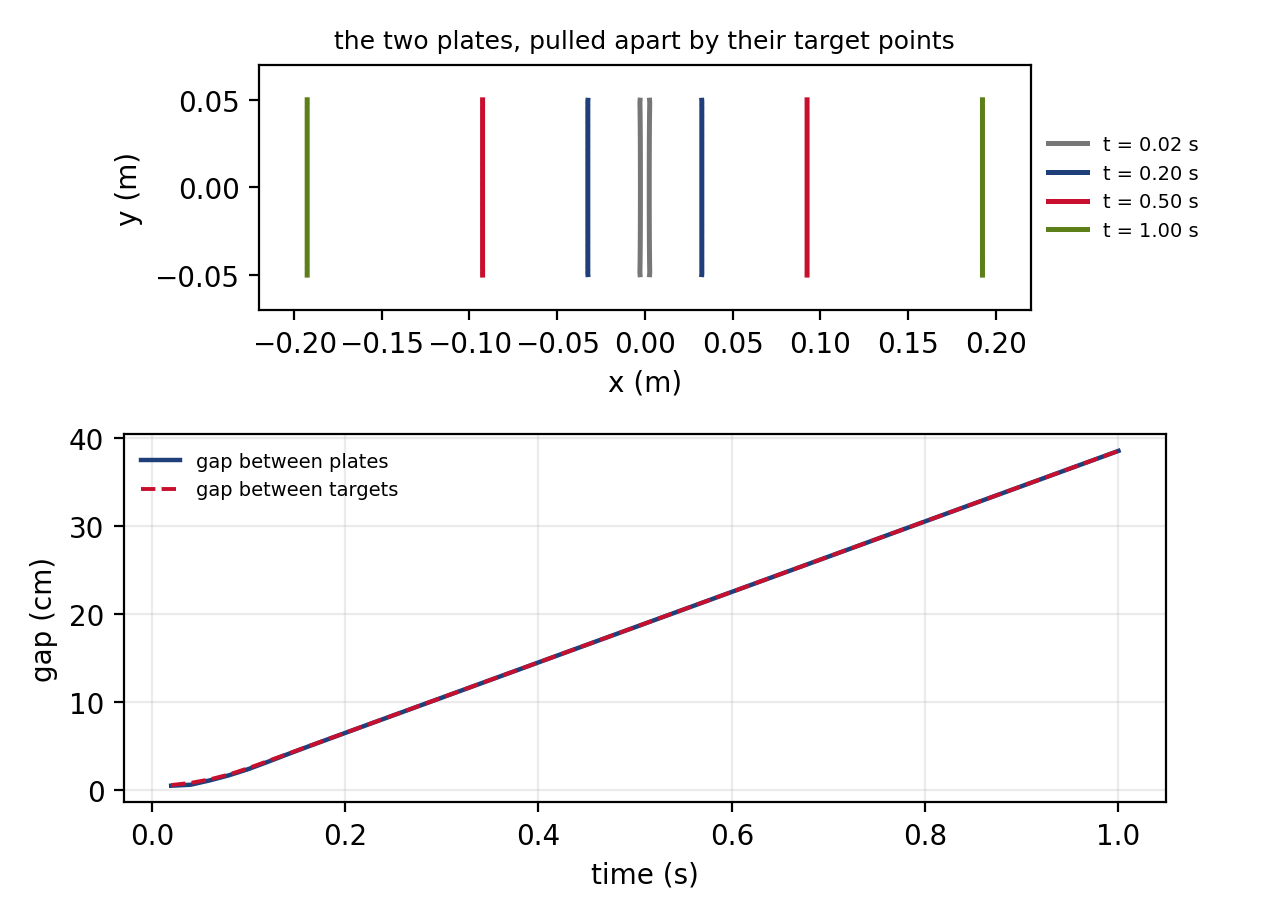
\includegraphics[width=\linewidth,height=0.66\textheight,keepaspectratio]{ch9a-plates}
\end{column}
\begin{column}{0.48\textwidth}
\scriptsize Top: the plates at four times; bottom: the gap between them against the gap between their targets.
\begin{itemize}
  \item the gap grows from $0.5$ cm to $38.5$ cm in 1 s, and the two curves are indistinguishable: the plates follow their targets to four digits (the targets' gap is $0.005 + 2\times0.19 = 0.385$ m at $t = 1$ s);
  \item the plates stay straight and vertical: every point is tethered, so the beams and springs have nothing to do. Tether only some points (the README's suggestion: write fewer lines into the \code{.target} files) and the plates bend as they are dragged, like the leaf of chapter 8a;
  \item the fluid between them is sucked in as they separate and pushed out ahead of them (the 2015--2020 picture, redrawn in chapter 26 from the \code{viz\_IB2d} output).
\end{itemize}
\scriptsize \code{DT = 1e-4} runs; \code{5e-5} gives the same gap and forces to 4 digits at $t = 0.2$ s; \code{2e-4} stops after 7 steps with \code{Time step size change encountered} (README).
\end{column}
\end{columns}
\sourcecredit{IB/07 with IBAMR 0.19.0, shipped input (1 s); \code{tools/ch9a\_figures.py}. The course version ran 2 s with \code{DT = 1e-6}.}
\end{frame}

% 23
\begin{frame}[fragile]{Stretching and shrinking plates (the 2015--2016 exercise)}
\label{fr:stretch}
\begin{columns}[T,onlytextwidth]
\begin{column}{0.5\textwidth}
\scriptsize ``You can comment out where you move the plates in \code{update\_target\_point\_positions}, and remove the comment from \code{update\_springs}. The code in \code{update\_springs} will make one plate stretch and the other shrink.''
\begin{lstlisting}[style=cpptiny]
// the exercise's code, with the copy bug fixed (a reference, not a copy)
for (std::vector<double>& spring : spring_spec->getParameters())
{
    if (plate2d_left_lag_idxs.first <= lag_idx && lag_idx < plate2d_left_lag_idxs.second)
        spring[1] += 0.01 * dt;   // "you could make the left plate grow ..."
    if (plate2d_rght_lag_idxs.first <= lag_idx && lag_idx < plate2d_rght_lag_idxs.second)
        spring[1] -= 0.01 * dt;   // "... and the right shrink"
}
\end{lstlisting}
\scriptsize The 2016 slide ``Left stretch, right shrink'' showed the result: the left plate longer than the right, each with its pair of eddies. The figure is not in the GitHub copy of the lecture (the crosswalk notes it); chapter 26's VisIt recipe reproduces it from a run.
\end{column}
\begin{column}{0.48\textwidth}
\scriptsize \al{``Move and stretch? You do not want to move the boundaries with target points and stretch/shrink the plates at the same time. Why would this be problematic?''} (the 2015--2020 question.)
\vspace{1mm}

\scriptsize The answer: every point of each plate is tethered to a target that moves as a rigid body. If the springs then try to lengthen the plate, each point is pulled one way by its spring and the other by its tether, and the tether wins ($\kappa = 2000/\Delta s$ against $K/\Delta s$ with $K = 2000$: the same number, so they fight to a standstill, with forces of either sign on neighbouring points). The plate neither moves cleanly nor stretches, the fluid gets a noisy force field, and the time step may fail. To do both, tether \emph{one} point (or a few) and let the springs set the shape; or move the targets apart along the plate at the same rate as the rest lengths grow, which is the same thing said twice.
\vspace{1mm}

\scriptsize The shrinking plate has its own trap: a rest length that reaches zero. At $0.01$ m/s per spring and $\Delta s \approx 10^{-3}$ m that happens at $t = 0.1$ s; after that the springs push apart (slide \ref{fr:other}). The course ran it for 2 s.
\end{column}
\end{columns}
\end{frame}

% 24
\begin{frame}{Can structures be connected? What 0.19.0 allows}
\label{fr:connect}
\small The 2014--2020 lectures said ``I don't think you can connect springs between them.'' Checked against the initializer:
\begin{itemize}
  \item A \code{.spring} (or \code{.beam}, \code{.xspring}) file names points by their index \emph{within that structure's} \code{.vertex} file; \code{IBStandardInitializer} adds the structure's offset when it builds the global numbering. There is no syntax for ``point 5 of the other structure'', so \al{files cannot join two structures}. The statement was right.
  \item Three ways around it:
  \begin{enumerate}
    \item \al{one structure, several parts}: put both plates in one \code{.vertex} file and join them with springs in the one \code{.spring} file; use the index ranges you know (points 0--102 are the left plate) in the update function instead of \code{getLagrangianStructureIndexRange};
    \item \al{the glue}: coincident points (slide \ref{fr:multi}), when the joint is a weld;
    \item \al{code}: \code{IBRedundantInitializer} (chapter 6) builds structures and their springs in \code{main.cpp} with explicit global indices, and a custom force (chapter 9b) can act between any two points.
  \end{enumerate}
\end{itemize}
\end{frame}

% 24b
\begin{frame}{Several structures or one with parts?}
\label{fr:connect2}
\scriptsize
\begin{tabular}{@{}L{0.3\textwidth}L{0.3\textwidth}L{0.3\textwidth}@{}}
\toprule
 & several structures & one structure with parts\\
\midrule
files & one set per structure, listed in \code{structure\_names} & one set; the parts are index ranges you know from the generator\\
springs and beams between the parts & impossible through files & ordinary lines of the \code{.spring} and \code{.beam} files\\
per-structure settings (\code{level\_number}, \code{uniform\_*}, \code{posn\_shift}, \code{length\_scale\_factor}; chapter 6) & each has its own & shared\\
telling the parts apart in code & \code{getLagrangianStructure}\allowbreak\code{IndexRange(k, ln)} & your own index arithmetic (and the generator's comments)\\
VisIt (chapter 26) & one Lagrangian mesh per structure in \code{lag\_data.visit} & one mesh\\
forces (chapter 11) & \code{integral\{F\}} is the sum over all; per-structure sums need the ranges & the same\\
\bottomrule
\end{tabular}

\vspace{2mm}
\small Use several structures when they are separate bodies with separate motions (two plates, a row of cylinders and a wall, a heart and its valves); use one structure with parts when they are joined and the joint carries force (a fin on a body, a valve leaflet on a tube). Coincident points (slide \ref{fr:multi}) join two structures without force, which is enough for a hinge that only transmits position.
\end{frame}

% 25
\begin{frame}[fragile]{Prescribed paths from data: interpolating between two states}
\label{fr:interp}
\begin{columns}[T,onlytextwidth]
\begin{column}{0.5\textwidth}
\footnotesize The 2015 MATH 769 lectures added two of Nick Battista's examples: ``Moving a cylinder in 2D'' (a complete process: create the geometry files, create coordinate \code{.txt} files to be read in by \code{update\_target\_point\_positions.C}, change the code accordingly, \code{make main2d}, run) and ``Moving (interpolating) between two states''. Their zip files lived on a UNC web page that no longer exists; the method survives.
\begin{lstlisting}[style=cpptiny]
// the pattern: targets move from state A to state B over a time T
// X_A, X_B: vectors of positions read once from two files (static, filled on the first call)
const double s = std::min(current_time / T, 1.0);          // or a smooth ramp, 0.5*(1 - cos(pi*s))
X_target[0] = (1 - s) * X_A[lag_idx][0] + s * X_B[lag_idx][0];
X_target[1] = (1 - s) * X_A[lag_idx][1] + s * X_B[lag_idx][1];
\end{lstlisting}
\end{column}
\begin{column}{0.48\textwidth}
\footnotesize Here the target is \al{set}, not shifted, so the function must know the two states; read them on the first call (a \code{static} flag) from files written by the same generator that wrote the \code{.vertex} file, in the same point order. The 2015 ``moving a cylinder'' example did exactly this with coordinate \code{.txt} files.
\vspace{1mm}

\footnotesize The two 2015 examples are the simplest form of \al{data-driven kinematics}: the structure does not compute its motion, it is told it, frame by frame. Notes on using the pattern: next slide.
\end{column}
\end{columns}
\end{frame}

% 25b
\begin{frame}{Interpolating between states: notes on the pattern}
\label{fr:interp2}
\footnotesize
\begin{itemize}
  \item A smooth $s(t)$ (the cosine ramp) avoids the impulsive start; a periodic $s(t) = \tfrac12(1 - \cos 2\pi f t)$ makes the structure go back and forth between the states at frequency $f$: a flapping wing from two drawn positions, the simplest kinematics. The frequency is the Strouhal number's $f$ (chapter 8b).
  \item More than two states: interpolate between consecutive frames of a digitized motion, $\mathbf{X}_{\mathrm{target}} = (1-s)\mathbf{X}_k + s\mathbf{X}_{k+1}$ with $k$ and $s$ from the time; chapter 1b's geometry pipeline ends with exactly such files, one per frame, in one point order.
  \item The states must have the \emph{same number of points in the same order}; a generator that writes all frames from one parametrization guarantees it. A digitized outline with a varying number of points must be resampled first.
  \item Setting targets rather than shifting them is robust to restarts (the position depends on the time only) and to a changed \code{DT}; shifting accumulates round-off and depends on the step history, which is harmless for a ramp but not for a long periodic motion.
  \item IB2d does this with its \code{update\_target\_point\_positions} script in MATLAB or Python (chapter 4c); the logic is identical and a good place to prototype.
\end{itemize}
\vspace{1mm}
\small This is how the lab's insect-wing and jellyfish kinematics were driven (Part VI); the valveless-pump set-up of chapter 36 uses the shift form with a travelling wave.
\end{frame}

% 26
\begin{frame}[fragile]{Parameters: out of the code and into the input file}
\label{fr:params}
\begin{columns}[T,onlytextwidth]
\begin{column}{0.5\textwidth}
\footnotesize The examples keep \code{V} and \code{time\_to\_acc} as \code{static const} numbers in the update function, as the course did. A sweep then means editing and rebuilding for every value. The better way, used by the pump set-up of chapter 36 and recommended there: read them from \code{input2d}.
\begin{lstlisting}[style=cpptiny]
// main.cpp: read once, pass down
const double V = input_db->getDouble("V_PLATES");
const double t_acc = input_db->getDouble("T_ACC");
...
update_target_point_positions(patch_hierarchy, l_data_manager, loop_time, dt, V, t_acc);
\end{lstlisting}
\begin{lstlisting}[style=input]
// input2d
V_PLATES = 0.2      // speed of the plates after the ramp (m/s)
T_ACC    = 0.1      // ramp time (s)
\end{lstlisting}
\end{column}
\begin{column}{0.48\textwidth}
\footnotesize
\begin{itemize}
  \item add the two arguments to the function and its header; \code{input\_db} is the top-level database \code{main.cpp} already holds (chapter 3);
  \item or pass the whole database (\code{Pointer<Database> db}) and let the function read what it needs;
  \item then a job array over \code{V\_PLATES} (chapter 8a) needs no rebuild, and the value is recorded in the input file of each run instead of in a binary.
\end{itemize}
\footnotesize Either way, keep the motion's \emph{units} in the comment: the speed is in m/s because the box is in metres; a dimensionless input (chapter 8b) would say ``in units of $U$''.
\vspace{1mm}

\footnotesize The same holds for \code{growth\_rate} in \code{update\_springs.cpp}, and for the frequency of any oscillating motion.
\end{column}
\end{columns}
\end{frame}

% 27
\begin{frame}{Time step and stiffness with moving targets}
\label{fr:dt}
\small A target point is a stiff spring, and a moving one must be stiff enough to drag the structure through the fluid without lagging (slide \ref{fr:cyl2}). The stiffness sets the time step (chapters 5 and 8a):
\vspace{1mm}

\scriptsize
\begin{tabular}{@{}L{0.18\textwidth}L{0.18\textwidth}L{0.2\textwidth}L{0.34\textwidth}@{}}
\toprule
example & $\kappa$ (file) & \code{DT} & measured (READMEs)\\
\midrule
IB/04 cylinders & $4.1\times10^6$ & $2\times10^{-5}$ & the largest step that runs; $5\times10^{-5}$ stops within a few steps\\
IB/07 plates & $2.04\times10^6$ & $10^{-4}$ & $5\times10^{-5}$ identical to 4 digits; $2\times10^{-4}$ stops after 7 steps\\
IB/02 channel walls & $2.05\times10^6$ & $10^{-4}$ & fixed targets; runs\\
IB/08 fibre (3D) & $3.2\times10^4$ & $10^{-5}$ & fixed targets; with \code{TARGET\_VELOCITY = 0.05} the run is unstable, $0.01$ runs\\
\bottomrule
\end{tabular}

\vspace{1mm}
\footnotesize
\begin{itemize}
  \item The lag is $F/\kappa$ and the step is $\propto 1/\sqrt{\kappa}$: a stiffness ten times smaller gives ten times the lag and three times the step. For a rigid body on a path, a lag of a tenth of a cell is usually fine; the cylinders are a thousand times stiffer than that.
  \item \code{error\_on\_dt\_change = TRUE} turns a step the integrator cannot take into the abort \code{Time step size change encountered} (chapter 5): the symptom of a target too stiff for \code{DT}, or a target moved too far in one step.
  \item Damping ($\eta$, chapter 8a's estimate) tames a target point that rings after a sudden change of its path; the examples use none.
\end{itemize}
\end{frame}

% 28
\begin{frame}{Checking that a prescribed motion is being followed}
\label{fr:check}
\small Four checks, in order of cost:
\begin{enumerate}\footnotesize
  \item \al{Print}: a \code{pout} of one target position and the corresponding point every few hundred steps (rank 0 only, or the output interleaves); the difference is the lag.
  \item \al{The force line}: \code{integral\{F\}} (chapter 11) is the sum of the tether forces, which is the force the fluid exerts on the structure. For a body on a path it should look like drag: a ramp-up while the body accelerates, then a steady or slowly changing value (IB/04: $594.8$ N/m at the end of its acceleration, $0.10$ s, falling to $238.9$ at $0.2$ s as the fluid around the row starts to move); a force that grows without bound or oscillates at the step frequency means the targets are fighting something (slide \ref{fr:stretch}) or the step is too large.
  \item \al{The positions}: the \code{X.*} files against the path, as in the figures of this chapter (\code{tools/ch9a\_figures.py}; chapter 11 has the reader). This is the check that catches the copy bug: a fibre whose length does not change.
  \item \al{VisIt}: the \code{lag\_data.visit} mesh at several times, and the velocity field around it (chapter 26); a structure that moves while the fluid does not is a tether without a kernel (wrong \code{level\_number}, chapter 6).
\end{enumerate}
\vspace{1mm}
\begin{punchbox}
\small Do the first two on a two-step run before anything longer: a prescribed motion that is wrong in the first step is wrong in all of them, and a run of twenty thousand steps tells you nothing a run of two did not.
\end{punchbox}
\end{frame}

% 29
\begin{frame}{What can go wrong}
\label{fr:wrong}
\scriptsize
\begin{tabular}{@{}L{0.3\textwidth}L{0.62\textwidth}@{}}
\toprule
The mistake & What happens\\
\midrule
a copy instead of a reference (\code{double r = ...[k][1]; r += ...}) & nothing changes, no error, no warning; the springs never grow (slide \ref{fr:copybug}). The same for \code{Point X = ...} instead of \code{Point\& X}\\
ghost nodes left out of the loop & correct on one process; in parallel, points near patch boundaries keep old targets and the structure tears or lags there (slide \ref{fr:loop})\\
velocity added instead of displacement (\code{X\_target[1] += V}) & the target jumps $V$ per step, $10^4$ times too far; the structure explodes or the run aborts at once\\
the wrong structure index & the other structure moves; or none, if the index does not exist (the range is empty)\\
the file not in \code{add\_executable} & \code{undefined reference to `update\_target\_point\_positions'} at link time; the header included but the function never built\\
edited the function, forgot to rebuild & the old motion runs; check the binary's time stamp or add a \code{pout} line\\
targets moved through a wall or out of the box & the points follow, and leave the domain: an abort at the next regrid (chapter 7)\\
$\kappa$ raised, \code{DT} not lowered & \code{Time step size change encountered} in the first steps (slide \ref{fr:dt})\\
moving targets and changing rest lengths of the same points & the tethers and springs fight; noisy forces, no clean motion (slide \ref{fr:stretch})\\
a rest length driven below zero & the spring becomes repulsive; keep rest lengths positive (slide \ref{fr:other})\\
\code{getParameters()[0]} only & fine on a chain; on a network a master of several springs changes only its first (slide \ref{fr:springs})\\
\bottomrule
\end{tabular}
\end{frame}

% 30
\begin{frame}{Homework}
\label{fr:hw}
\begin{columns}[T,onlytextwidth]
\begin{column}{0.55\textwidth}
\scriptsize From the 2015--2020 courses and the READMEs (Appendix C collects the full set):
\begin{enumerate}
  \item IB/04: make the row move sideways instead of up, and change \code{V} or \code{time\_to\_acc}; predict the lag from $\kappa$ and \code{integral\{F\}} before you measure it.
  \item IB/07: move only one plate; then tether only the middle point of each plate and watch them bend as they are dragged.
  \item IB/07: the stretch-and-shrink exercise with the corrected code; stop before the right plate's rest length reaches zero, and explain why ``move and stretch'' at once is a bad idea.
  \item IB/06: make the rest length oscillate, \code{A*sin(2*PI*f*t)*dt} per spring, with the 2018 numbers ($A = 0.00049$, $f = 1$ Hz); then halve \code{growth\_rate} in the original and report when the fibre buckles.
  \item Write a function that moves a structure between two drawn states (slide \ref{fr:interp}) and drive IB/03's leaf with it instead of the stream.
\end{enumerate}
\end{column}
\begin{column}{0.43\textwidth}
\begin{punchbox}
\scriptsize What to hand in (the 2018--2020 pattern): the changed lines of the update function, the \code{CMakeLists.txt} line, one VisIt frame per case, and the check of slide \ref{fr:check} that shows the motion was followed.
\end{punchbox}
\scriptsize Extension: move \code{V} and \code{time\_to\_acc} into the input file (slide \ref{fr:params}) and run a job array over three speeds (chapter 8a).
\end{column}
\end{columns}
\end{frame}

% 31
\begin{frame}{Rules of thumb}
\label{fr:thumb}
\footnotesize
\begin{itemize}
  \item Target points prescribe a \emph{force toward} a path, not a velocity; the lag is $F/\kappa$ and the price of a small lag is a small \code{DT}.
  \item Shift the targets by (speed at \code{current\_time}) $\times$ \code{dt}, before \code{advanceHierarchy}; ramp the speed from zero.
  \item Loop over local \emph{and} ghost nodes; test the spec pointer for \code{nullptr}; take every accessor as a reference.
  \item A spring belongs to its lower-numbered point; \code{getParameters()[k][0]} is the file stiffness, \code{[k][1]} the rest length; change every \code{k}.
  \item Several structures: one set of files each, listed in \code{structure\_names}; that order is the numbering; the index range of each structure (\code{getLagrangian\-Structure\-Index\-Range}) tells them apart.
  \item Files cannot join structures; one structure with parts, coincident points, or code can.
  \item Do not move targets and change rest lengths of the same points at once; keep rest lengths positive.
  \item Both source files in \code{add\_executable}; rebuild after every edit; parameters into the input file for sweeps.
  \item Two steps, print one target and its point, read \code{integral\{F\}}, then the long run.
\end{itemize}
\end{frame}

% 32
\begin{frame}{Summary}
\label{fr:summary}
\footnotesize
\begin{enumerate}
  \item At run time each target point and each spring is a small object attached to its master point, holding $\kappa$, $\eta$, $\mathbf{X}_{\mathrm{target}}$ or the spring parameters, with accessors that return references. Prescribed motion in IB is changing those numbers before each step.
  \item The update function receives the hierarchy, the \code{LDataManager}, the time and the step; it loops over local and ghost nodes of the finest level, asks each for its spec, and shifts the target (or the rest length) by a rate times \code{dt}. \code{main.cpp} calls it before \code{advanceHierarchy}, and \code{CMakeLists.txt} lists the file.
  \item The cylinders follow their targets to half a micrometre at $\kappa = 4\times10^6$ and \code{DT = 2e-5}; the plates' gap tracks the targets' to four digits; the fibre lengthens six-fold and buckles into waves once drag compresses it, which it did not do in the course's run because the rest length was changed on a copy.
  \item Several structures are several sets of files in \code{structure\_names}, numbered in that order; the index ranges tell them apart; files cannot join them, but one structure with parts, coincident points or code can.
  \item Check with a print, the force line, the position files and VisIt, on a short run first.
\end{enumerate}
\begin{homebox}
\footnotesize Next, chapter 9b: forces you write yourself, custom spring laws through \code{registerSpringForceFunction}, applied external forces, and active pumping.
\end{homebox}
\end{frame}

% 33
\begin{frame}{What changed since the older course notes}
\label{fr:changed}
\small
\begin{itemize}
  \item The API is the 0.19.0 one throughout (\code{getNodeDataItem}, \code{IBTK::Point}, \code{getParameters}, \code{LMesh} nodes, \code{.cpp}, CMake), with the 2009--2020 spellings in a table so that old code can be read; the 2009 listing from the 2012 deck is kept for that purpose.
  \item The copy-versus-reference bug of the course's \code{update\_springs} (2013--2020) is named, explained and fixed; the series' IB/06 grows and buckles, and the figure shows it.
  \item Ghost nodes, the half-open index range, the structure numbering (0--102, 103--205) and the parameters-in-the-input-file pattern are new; so are the three measured figures, the lag table and the time-step table.
  \item ``I don't think you can connect springs between them'' is answered from the initializer, with the three ways around it; the ``glue'' of coincident points is explained; the ``Move and stretch?'' question is answered.
  \item The 2015 Battista examples (moving a cylinder, interpolating between two states) are kept as the method; their UNC download links are dead.
  \item The course comments that called the cylinders and plates ``the wing'' and said the row moves ``left or right'' are corrected in the examples; sakai, nemo and Google Code links are gone; the 2013 slide's server password is not reproduced.
\end{itemize}
\end{frame}

% 34
\begin{frame}{Recordings (listed, not incorporated)}
\label{fr:videos}
\small The front matter's video list (chapter 0.1) has these recordings of this material:
\vspace{1mm}

\scriptsize
\begin{tabular}{@{}L{0.5\textwidth}L{0.14\textwidth}L{0.3\textwidth}@{}}
\toprule
Recording & Date & Course\\
\midrule
\code{5-Video-SpringsTargetsPart1.mp4}, \code{Part2.mp4} & 2018-02-14 & MATH 769 (IBAMR Part 1: Getting Started)\\
\code{6-Video\_IBAMRTutorial\_}\allowbreak\code{MultipleBoundaries\_}\allowbreak\code{DomainSize\_InputFile.mp4}, \code{Part2.mp4} & 2018-03-19 & same (also covers chapter 7's domain sizes)\\
\code{Lecture 5 - Moving immersed boundaries.mp4} & 2020-05-19 & 2020 Zoom lectures\\
\code{IBAMR-MovingTarget-ChangeSprings.mp4} & 2024-07-28 & 2024 IBAMR videos\\
\bottomrule
\end{tabular}

\vspace{2mm}
\small The 2018 recordings follow the 2017 ``5 -- Changing Target Positions and Springs'' and ``Multiple Boundaries'' decks (with the copy bug on screen); the 2020 and 2024 ones follow the 2020 Lecture 5. The IBFE tethered-plate video of 2024 belongs to Part IV.
\end{frame}

% 35
\begin{frame}{References}
\label{fr:refs}
\scriptsize
\begin{itemize}
  \item IBAMR 0.19.0: \code{ibtk/include/ibtk/LDataManager.h} (the documented example of moving target points and of reading positions), \code{LMesh.h}, \code{LNode.h}, \code{LNodeIndex.h}; \code{include/ibamr/IBTargetPointForceSpec.h}, \code{IBSpringForceSpec.h}, \code{IBBeamForceSpec.h}; \code{src/IB/IBStandardInitializer.cpp} (structure numbering), \code{IBStandardForceGen.cpp} (the forces); \code{ibtk/include/ibtk/HierarchyIntegrator.h} (the preprocess callback). \url{https://github.com/IBAMR/IBAMR}
  \item IBAMR FAQ: \url{https://github.com/IBAMR/IBAMR/wiki/FAQ}; class documentation: \url{https://ibamr.github.io/docs}.
  \item The examples of this series: IB/04 moving cylinders, IB/06 growing springs, IB/07 moving plates (each with \code{update\_*.cpp}, \code{.h}, \code{main.cpp}, \code{CMakeLists.txt} and a README with the measured time steps and motions); \code{tools/ch9a\_figures.py} for the figures.
  \item B. E. Griffith's \code{moving\_plates} example (2009), as reproduced in the January 2012 tutorial; now \code{examples/IB/explicit} in the IBAMR tree holds the current moving-structure examples (chapter 15).
  \item Sources: \emph{Immersed boundary tutorial continued} (January 2012); \emph{Changing spring lengths, stiffnesses and target points} and \emph{IBAMR with multiple boundaries} (MATH 769, February 2013); \emph{MATH 769 Lecture 8} and \emph{Lecture 12} (2015); \emph{4 -- Changing Target Positions and Springs} and \emph{5 -- Multiple Boundaries} (public folder, 2014--2016); \emph{5 -- IBAMR Tutorial: Changing Target Positions and Springs} (MBI, 2017); \emph{Lecture 5 -- IBAMR Tutorial: Changing Target Positions and Springs} (2020, edited 2024).
\end{itemize}
\end{frame}

\end{document}
